\documentclass[10pt]{exam}
\usepackage[utf8]{inputenc}

\usepackage[margin=1in]{geometry}
\usepackage{amsmath,amssymb}
\usepackage{multicol}
\usepackage{multirow}
\usepackage{graphicx}
\usepackage{tikz}
\newcommand{\clase}{CÁLCULO INTEGRAL}
\newcommand{\examnum}{Parcial 2}
\newcommand{\examdate}{ 16 de abril de 2019}
\newcommand{\timelimit}{120 Minutos}
\definecolor{Micolor1}{gray}{0.7}
\pagestyle{head}
\firstpageheader{\Large\sc\clase}{}{\sc\examnum}
\runningheader{\sc\clase}{}{\sc\examnum\ - P\'agina \thepage\ de \numpages}
\runningheadrule


\begin{document}
\vspace{1.5cm}
\begin{tabular}{ll}
\multirow{5}{*}{
\includegraphics[scale=0.28]{Sabana1.png}}
%&\textbf{Examen Final}\\
& \large\hspace{0.5cm}Nombre: \makebox[2.7in]{\hrulefill}\vspace{0.2cm}\\
& \large\hspace{0.5cm}Fecha:\textbf{\examdate} \vspace{0.2cm}\\
& \large\hspace{0.5cm}Tema: A \vspace{0.2cm}\\
& \large\hspace{0.5cm}Profesor: \makebox[2.7in]{\hrulefill}\vspace{0.2cm}\\
%& \large\hspace{1.0cm}Tiempo límite: \textbf{\timelimit}}
\end{tabular}\\
\rule[2ex]{\textwidth}{2pt} 
\begin{itemize}
\scriptsize{\item \textbf{No se permite el uso de elementos electrónicos, smartwatches, etc. La presencia de cualquier equipo de comunicación en el entorno del examen es considerado intento de fraude. Éste o cualquier otro intento de fraude implica cero en el examen y se reporta a la facultad.}
    \item \textbf{La comprensión del examen es parte de la evaluación, por tanto, no se responden preguntas.} 
    \item \textbf{Se evalúa procedimiento y/o justificación, por tanto, sea claro y ordenado.}
   % \item \textbf{Este examen contiene \numpages\ páginas y \numquestions\ preguntas.  El Total de puntos en esta prueba es de \numpoints}
   }
\end{itemize} 

%\begin{center}
%\textbf{Tabla de Puntos (No marcar. Uso exclusivo del profesor)}\\
\addpoints
%\gradetable[v][questions]
%\end{center}

\noindent
\rule[2ex]{\textwidth}{2pt}


\begin{enumerate}
\normalsize
\setlength{\columnsep}{10mm}



\item \textbf{[Distancia y velocidad]}  Juan y Mariana viajan en un carro con el velocímetro averidado. Para determinar la distancia que recorren entre 2pm y las 3pm, Mariana (la pasajera) toma lecturas del velocímetro cada 5 minutos:

\begin{center}

%\begin{table}[]
\begin{tabular}{|l|l|l|l|l|l|l|l|l|l|l|l|l|l|}
\hline
Minutos después de 2pm  & 0  & 5  & 10 & 15 & 20 & 25 & 30 & 35 & 40 & 45 & 50 & 55 & 60 \\ \hline
Lectura del velocímetro (km/h) & 45 & 48 & 37 & 39 & 55 & 60 & 60 & 55 & 50 & 67 & 58 & 45 & 49 \\ \hline
\end{tabular}
%\end{table}
\end{center}
\begin{enumerate}
    \item Utilice la regla del trapecio para estimar la distancia total recorrida entre las 2pm y las 3pm. \hfill{[B2]}
    
   
    \item Google Maps  asegura que la distancia recorrida ha 55 km .  ¿Cuál fué el error (inexactitud) que se cometió en el inciso (a)?  \hfill{[B3]}
    
\end{enumerate}

\item Se proyecta que $t$ años a partir de ahora el tamaño de la población de cierta ciudad cambiará a una velocidad $n^{\prime}(t)=t\ln{(t+1)}$ milones de personas por año.  \hfill{[B1]}

\begin{center}
    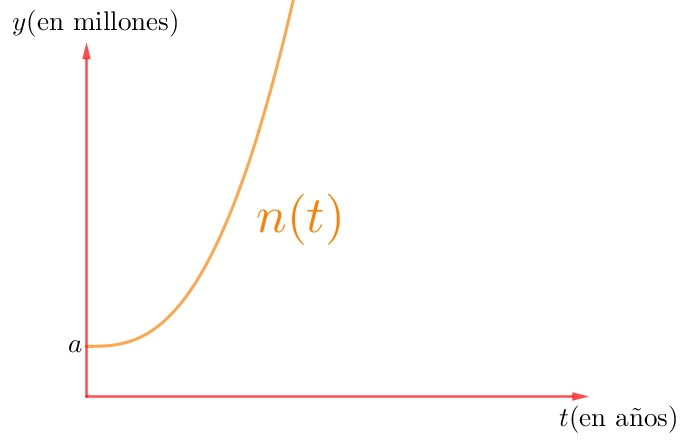
\includegraphics[scale=1.3]{PoblacionA.png}
\end{center}
\begin{enumerate}
    \item ¿Cuál es el tamaño de la población en (millones) en este momento?  \hfill{[B1]}



    
    \item ¿Cuál es el tamaño de la población  (en millones) después de 5 años a partir de ahora?\hfill{[B2]}
    

\end{enumerate}



\item Al hacer un cambio de variable sobre \[\int_1^{4}\frac{dy}{2\sqrt{y}(1+\sqrt{y})}\, dx\] se puede sustituir como: \hfill{[C2]}


\begin{multicols}{4}
\begin{enumerate}
    \item \(\displaystyle{\int_4^1 \frac{du}{u^2}}\)

    \item \(\displaystyle{\int_2^3 \frac{du}{u}}\)
    
    \item \(\displaystyle{\int_2^3 \frac{du}{u^2}}\)

    \item \(\displaystyle{\int_1^4 \frac{du}{u^2}}\)
\end{enumerate}
\end{multicols}{}
\item Al hacer un cambio de variable sobre \[\int_4^{40}x\sqrt{2x+1}\, dx\] se puede sustituir como: \hfill{[C2]}

\begin{multicols}{4}
\begin{enumerate}
    \item \(\displaystyle{\int_3^9 \frac{(u^2-1)u^2}{2}\, du}\)
    \item \(\displaystyle{\int_3^8 \frac{(u^2-1)u^2}{2}\, du}\)
    \item \(\displaystyle{\int_9^{80} \frac{(u+1)\sqrt{u}}{4}\, du}\)
    \item \(\displaystyle{\int_9^{81} \frac{(u+1)\sqrt{u}}{4}\, du}\)
\end{enumerate}
\end{multicols}{}


\item Un árbol ha sido trasplantado y después de \(t\) años está creciendo a un ritmo de \[r^{\prime}(t)=\frac{1}{t^2+7t+12},\,\,\,\,\,\,\, t\geq 0\]

metros por año.  Si al momento de ser trasplantado el árbol midió $2\ln(2)$ metros, ¿cuánto medirá en tres años?
\end{enumerate}


\end{document}
